
\chapter{Statistical Learning}
\hl{reference statistical learning (voir mas1)}

This section do not cover all the formulas talk in the book since we already seen it in \emph{Modèle Linéaire en actuariat}. This section talk more about the analysis of some statistical model.

\section{Statistical Learning}

\paragraph{Prediction}
\begin{align*}
    \esp{Y - \hat{Y}} &= \esp{f(x) + \varepsilon - \hat{f}(x)}^2 \\
                      &= [f(x) - \hat{f}(x)]^2 + \variance{\varepsilon} \\
                      &= (\text{Réductible}) + (\text{Irreductible)}
\end{align*}

\paragraph{Inference}
We are often interested in understanding the way that Y is affected as $X_1,...,X_p$ is changing. Inference mean that we want to understand the relationship between X and Y, or more specifically, to understand how Y changes as a function of $X_1,...,X_p$ 
\begin{itemize}
    \item Which predictors are associated with the response?
    \item What is the relationship between the response and each predictor?
    \item Can the relationship between Y and each predictor be adequately summarized using a linear equation, or is the relationship more compli cated?
\end{itemize}

\subsection{How Do We Estimate f?}
\paragraph{Parametric Methods}
Parametric methods involve a two-step model-based approach.

\begin{enumerate}
    \item  First, we make an assumption about the functional form, or shape, of f. For example, one very simple assumption is that f is linear in X: \[ f(X) = \beta_0 + \beta_1 X_1 + ... + \beta_p X_p \]
    \item  After a model has been selected, we need a procedure that uses the training data to fit or train the model.enumarate
\end{enumerate}

The potential disadvantage of a parametric approach is that the model we choose will usually not match the true unknown form of f. If the chosen model is too far from the true f, then our estimate will be poor. We can try to address this problem by choosing flexible models that can fit many different possible functional forms for f. But in general, fitting a more flexible model requires estimating a greater number of parameters. These more complex models can lead to a phenomenon known as overfitting the data.

\paragraph{Non-parametric Methods}
No assumption about the form of f is made. 
\begin{itemize}
    \item \textbf{Advantage:} Fit the model more closly to the data points.
    \item \textbf{Disadvantage:} Since they do not reduce the problem of estimating f to a
small number of parameters, a very large number of observations (far more
than is typically needed for a parametric approach) is required in order to
obtain an accurate estimate for f.
\end{itemize}

\begin{figure}[!ht]
\centering
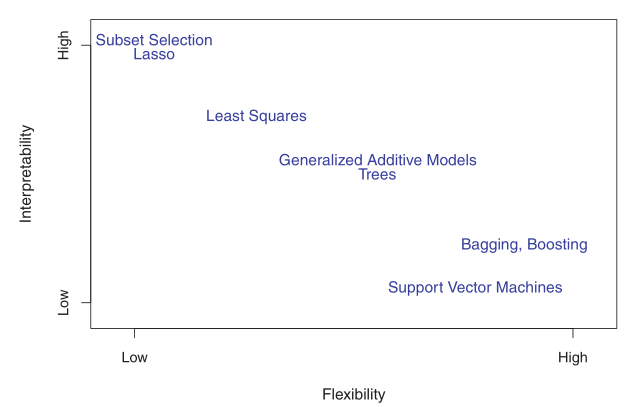
\includegraphics[scale=0.7]{src/StatisticalLearning/Trade-Off_Prediction-Interpretability.PNG}
\caption{A representation of the tradeoff between flexibility and interpretability, using different statistical learning methods. In general, as the flexibility of a method increases, its interpretability decreases.}
\end{figure}

\subsection{Measuring the Quality of Fit}
In the regression setting, the most commonly-used measure is the mean squared error (MSE), given by
\[ \mathrm{MSE} = \frac{1}{n} \sumn (y_i - \hat{f}(x_i))^2  \]
The MSE will be small if the predicted responses are very close to the true responses.

Note that regardless of whether or not overfitting has
occurred, we almost always expect the training MSE to be smaller than
the test MSE because most statistical learning methods either directly or
indirectly seek to minimize the training MSE.

\paragraph{Overfitting}
Overfitting refers specifically
to the case in which a less flexible model would have yielded a smaller
test MSE.

\paragraph{The Bias-Variance Trade-Off}
The equation below tells us that in order to minimize the expected test error,
we need to select a statistical learning method that simultaneously achieves
low variance and low bias. Note that variance is inherently a nonnegative
quantity, and squared bias is also nonnegative. Hence, we see that the
expected test MSE can never lie below Var(?), the irreducible error
\[ \esp{y_0 - \hat{f}(x_0)} \variance{\hat{f(x_0)}} + [ \mathrm{Bias}(\hat{f}(x_0))]^2 + \variance{\varepsilon} \]
\begin{itemize}
    \item \textbf{Variance} refers to the amount by which $\hat{f}$ would change if we estimated it using a different training data set.  In general, more flexible statistical methods have higher variance.
    \item \textbf{Bias} refers to the error that is introduced by approximating a real-life problem, which may be extremely complicated, by a much simpler model. Generally, more flexible methods result in less bias.
\end{itemize}

\begin{figure}[!ht]
    \centering
    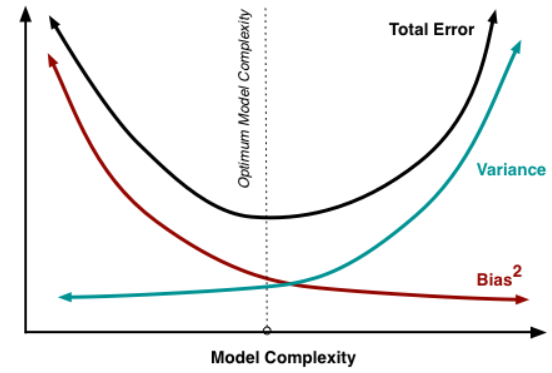
\includegraphics[scale=0.7]{src/StatisticalLearning/Trade-off_Variance-Bias.PNG}
    \caption{Bias-Variance trade-Off}
\end{figure}

\section{Linear Regression}

\subsection{Simple Linear Regression}
\paragraph{Definition}
\[ \hat{y} = \hatbeta_0 + \hatbeta_1 x \]
where the $\hatbeta$ are estimate using the \textbf{least squares} criterion.

\begin{figure}[!ht]
    \centering
    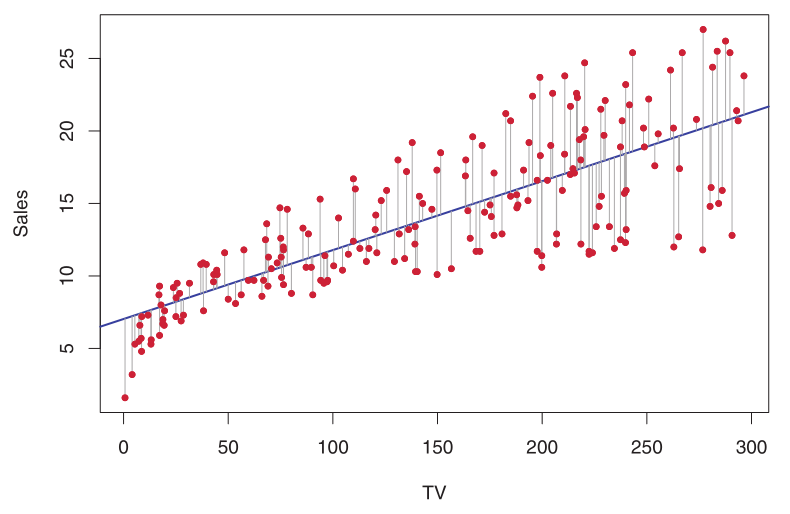
\includegraphics[scale=0.5]{src/StatisticalLearning/SimpleLinearRegression.PNG}
    \caption{Exemple of simple linear regression}
\end{figure}

\paragraph{Residual sum od squares}
We define the residual sum of square as
\[ \mathrm{RSS} = \mathrm{SSE} = \sumn \varepsilon_i = \sumn (y_i - \hat{y}_i)^2 \]

\paragraph{$R^2$ Statistic} 
For simple linear regression, $R^2 = \covar{X, Y}$.

Backward selection cannot be used if p > n, while forward selection can
always be used. Forward selection is a greedy approach, and might include
variables early that later become redundant. Mixed selection can remedy
this.

\section{Multiple Linear Regression}

\subsection{Potential Problems}
When we fit a linear regression model to a particular data set, many prob-
lems may occur. Most common among these are the following:

\paragraph{1. Non-linearity of the Data}
The linear regression model assumes that there is a straight-line relationship between the predictors and the response. If the true relationship is far from linear, then virtually all of the conclusions that we draw from the fit are suspect. In addition, the prediction accuracy of the model can be significantly reduced.

Residual plots are a useful graphical tool for identifying non-linearity. If the residual plot indicates that there are non-linear associations in the data, then a simple approach is to use non-linear transformations of the predictors, such as $\ln(X)$, $\sqrt{X}$, and $X^2$ , in the regression model.

\paragraph{2. Correlation of Error Terms}
An important assumption of the linear regression model is that the error terms, $\varepsilon_1,...,\varepsilon_n$ are uncorrelated. If in fact there is correlation among the error terms, then the estimated standard errors will tend to underestimate the true standard errors.

\begin{figure}[!ht]
    \centering
    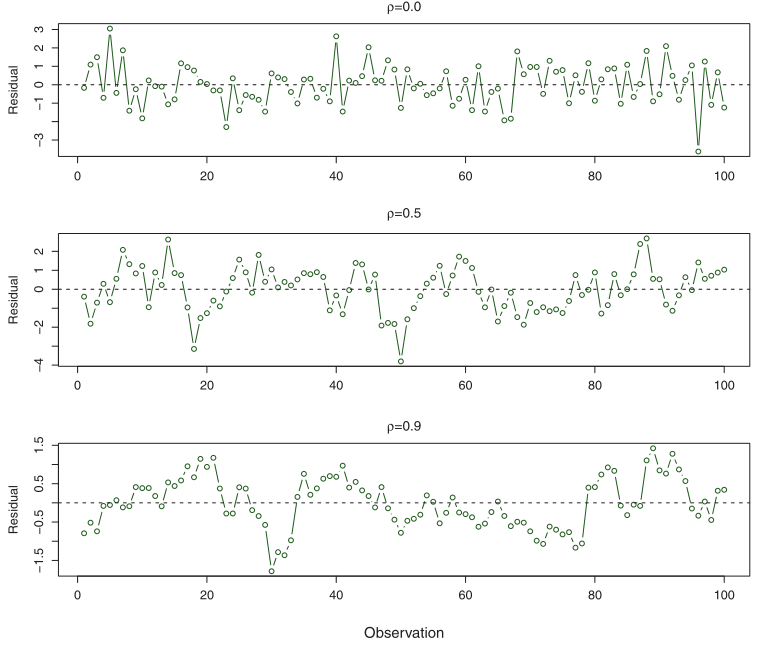
\includegraphics[scale=0.6]{src/StatisticalLearning/CorrelationInErrorTerms.PNG}
    \caption{Plots of residuals time series data sets with differing levels of correlation $\rho$ between error terms for adjacent time points. The graphs on top is good for linear regression}
\end{figure}

\paragraph{3. Non-constant Variance of Error Terms}
Another important assumption of the linear regression model is that the
error terms have a constant variance, $\variance{\varepsilon} = \sigma^2$. If not, we can recognize \textbf{heteroscedasticity} with a funnel shape in the residual plot.

\begin{figure}[!ht]
    \centering
    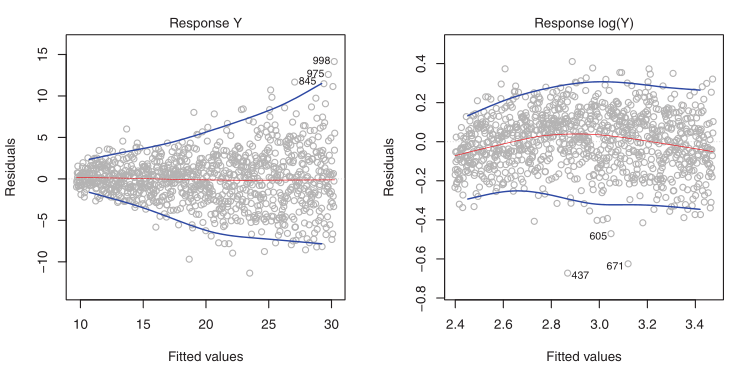
\includegraphics[scale=0.6]{src/StatisticalLearning/Heteroscedasticity.PNG}
    \caption{Residual plots. Left: The funnel shape indicates heteroscedasticity. Right: The predictor has been log-transformed, and there is now no evidence of heteroscedasticity.}
\end{figure}

 When faced with this problem, one possible solution is to transform the response Y using a concave function such as $\ln(Y)$ or $\sqrt{Y}$. Such a transformation results in a greater amount of shrinkage of the larger responses, leading to a reduction in heteroscedasticity. Sometimes, we can also use \textbf{weighted least squares}.

\paragraph{4. Outliers}
An outlier is a point for which $y_i$ is far from the value predicted by the model. Outliers can arise for a variety of reasons, such as incorrect recording of an observation during data collection.

\begin{figure}[!ht]
    \centering
    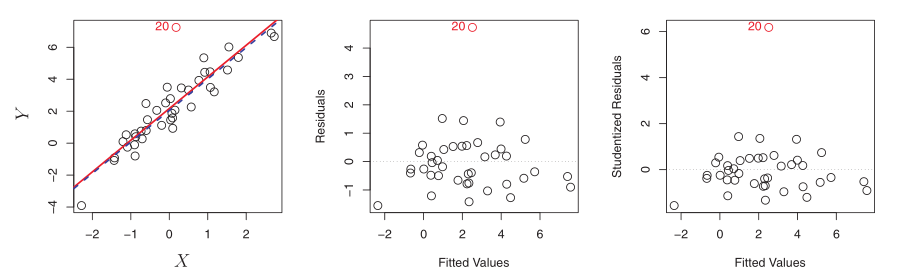
\includegraphics[scale=0.6]{src/StatisticalLearning/Outlier.PNG}
    \caption{Center: The residual plot clearly identifies the outlier. Right: The outlier has a studentized residual of 6; typically we expect values between -3 and 3.}
\end{figure}

Outlier can affect our MSE estimation, resolving in inadequate $R^2$ or confidence interval. We can remove the outlier to resolve this issue.

\paragraph{5. High Leverage Points}
In constrast of \emph{outlier} that are unusual $y_i$, leverage are unusual value of $x_i$. 

\begin{figure}[!ht]
    \centering
    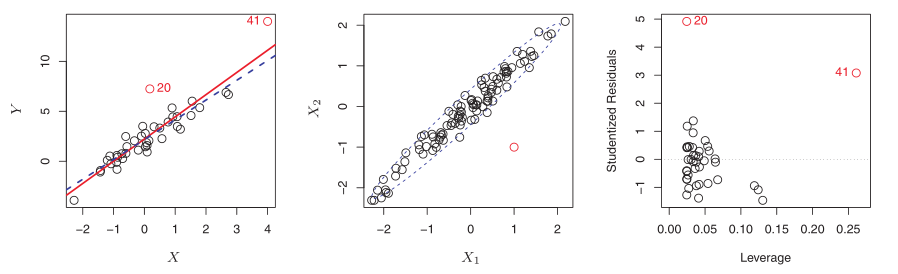
\includegraphics[scale=0.6]{src/StatisticalLearning/Leverage.PNG}
    \caption{Left: Observation 41 is a high leverage point, while 20 is not. The red line is the fit to all the data, and the blue line is the fit with observation 41 removed. Center: The red observation is not unusual in terms of its $X_1$ value or its $X_2$ value, but still falls outside the bulk of the data, and hence has high leverage. Right: Observation 41 has a high leverage and a high residual.}
\end{figure}

For simple linear regression, we can compute the leverage statistic define as
\[ h_i = \frac{1}{n} + \frac{(x_i - \bar{x})^2}{\sum (x_i - \bar{x})^2} \]
where $\frac{1}{n} < h_i < 1$ and $\sum h_i = \frac{(p+1)}{n}$.
So if a given observation has a leverage statistic that greatly exceeds $(p+1)/n$, hen we may suspect that the corresponding point has high leverage.

\paragraph{6. Collinearity}
Collinearity refers to the situation in which two or more predictor variables collinearity are closely related to one another.

\begin{figure}[!ht]
    \centering
    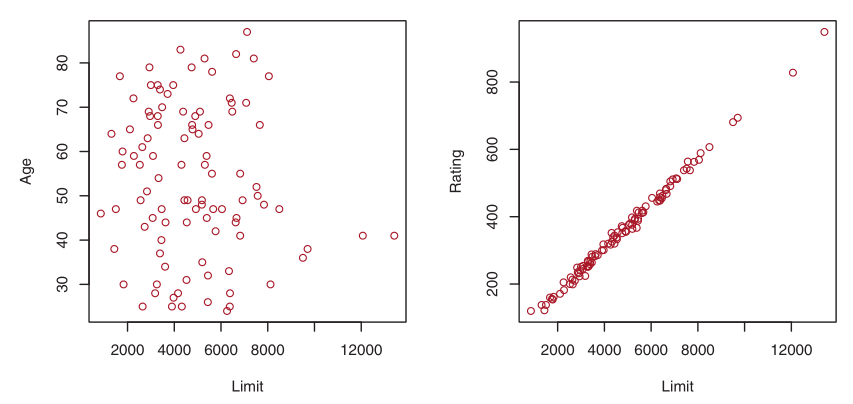
\includegraphics[scale=0.6]{src/StatisticalLearning/Collinearity.PNG}
    \caption{Left: A plot of age versus limit. These two variables are not collinear. Right: A plot of rating versus limit. There is high collinearity.}
\end{figure}

The presence of collinearity can pose problems in the regression context, since it can be difficult to separate out the individual effects of collinear variables on the response.

